\documentclass[12pt,a4paper]{article}

% Load preamble
\usepackage{preamble}

\begin{document}

% Frontpage
\title{%
  Take-home exam \\
  AP
}%
\author{Exam number 66}
%%\date{\today}%

\maketitle
\thispagestyle{empty}
\newpage
\setcounter{page}{1}

% Sections
\section*{The \texttt{appm} package manager}

\subsection*{Utility functions}
\paragraph{Version ordering}
It turns out that ordering versions as described in the assignment can be accomplished by simply deriving the \texttt{Ord} typeclass from \texttt{Version} and \texttt{VNum}. By doing this, I tell the compiler to use the default ordering on the contained \texttt{VNum} list. Each of the version numbers in the list will, by default, be compared by first comparing the number, and then the string. Each element of the two lists are compared, in order, until two version numbers numbers aren't equal, in which case the inequality determines the result of the comparison. Thus, the default ordering accomplishes what I set out to do with the \texttt{Version} type.

% The \texttt{merge} function works by computing the intersections of allowed version ranges for constraints on the same package. More specifically, when merging two constraint lists $c_1$ and $c_2$, I add each element of $c_2$ to $c_1$ iteratively. Each time, I perform a linear traversal of $c_1$; if I stumble upon a constraint on the same package, I merge the two individual constraints by computing the intersection of allowed versions and setting the flag, indicating whether the package is required or a conflict, to \texttt{True} if at least one of the flags was set beforehand.
%
% The claim that this will yield a fully reduced constraint list is based on the assumption that both individual lists are fully reduced. In fact, I only rely on the assumption that $c_1$ is fully reduced. In order to \textit{guarantee} a fully reduced solution, one could instead merge each element in \texttt{$c_1$ ++ $c_2$} into an initially empty list by the same approach.

\paragraph{Merging dependencies}
 The \texttt{merge} function works by computing the intersections of allowed version ranges for constraints on the same package. More specifically, when merging two constraint lists $c_1$ and $c_2$, I build a new constraint list $c'$ from scratch. Each element of $c_1$ and $c_2$ is added to $c'$ iteratively. Each time, I perform a linear traversal of $c'$; if I stumble upon a constraint on the same package along the way, I merge the two individual constraints by computing the intersection of allowed versions and setting the flag, indicating whether the package is required or a conflict, to \texttt{True} if at least one of the flags was set beforehand. If any intersection yields an empty range, there is no result.

 By building the new constraint list from scratch, I make sure that the resulting constraint list is fully reduced; if I simply merged each constraint of $c_2$ into $c_1$ and assumed $c_1$ itself to be fully reduced, I could potentially encounter some problems where this is not the case, i.e.\ when checking equivalence between dependencies of two different versions of the same package. The assumption may be reasonable since I merge them in the parser in an order that guarantees a fully reduced constraint list, but a more robust behaviour is in my opinion preferable.

\subsection*{Parsing \texttt{appm} databases}
I chose to use the Parsec parser combinator library since I have worked with it before. Furthermore, it is well documented and widely used. It generates reasonable error messages when parsing, and I like the overall layout of the combinator as a whole.

Only few intricacies occured when implementing the parser, in particular parsing and generating packages. Given the Parsec parser combinator, the rest has been more or less trivial; most of the requirements are addressed by simply adding a case or two to each parser.

\paragraph{Parsing and generating packages} The task is to parse a package in the database, but also to make sure that said record is well-formed given the criteria from the assignment. I achieve this by defining a custom data type, \texttt{Clause}, which denotes each type of valid clause in a package. When parsing a package, I parse all the clauses and generate a \texttt{Clause} list of these. I then check that these clauses collectively satisfy the constraints on the number of each type of clause. If all is as expected, I traverse the \texttt{Clause} list and accumulate a package. The dependendcies are generated by merging (using the \texttt{merge} function described in the previous section) each occurring constraint with the already accumulated dependencies in the package. If I'm not able to merge some constraints along the way, I throw an error.

I chose to do it this way since it eases the sanity check of a package and allows the user to define clauses in any arbitrary order. Furthermore, it is based on a simple, linear traversal of all clauses, which can be accomplished with our favourite bulk operators (\texttt{map}, \texttt{foldl}, etc.). All in all it seems to be the simplest and most effective solution for the given task.

\paragraph{Other stuff worth mentioning} To make keywords case insensitive I have chosen to simply parse each char of a string, convert it to lower case if applicable, generate a new string from these, and then match this string on the predefined keyword.

In order to correctly escape double quotes within a string, I parse arbitrary characters until I encounter a pair of double quotes. When this happens, I put one double quote in the string.

To parse dependencies, I first parse either the \texttt{"requires"}- or the \texttt{"conflicts"} keyword. Which of these is parsed determines the boolean flag in the resulting constraint. Then, the way the actual range is generated depends on this flag; if the flag is set, the resulting range is the \textit{intersection} of the two inequalities. If not, the range is the \textit{complement} of the two inequialities. That is,
\begin{align*}
  \texttt{requires bar >= 0, bar < 7}  & \ \ : \ \  \text{versions 0-7 are \it required} \\
  \texttt{conflicts bar < 0, bar >= 7} & \ \ : \ \  \text{versions 0-7 are \it allowed}
\end{align*}
Note that the inequalities are still inferred when no version numbers are specified explicitly. That is, \texttt{conflicts foo} sets an empty allowed range for \texttt{foo}, and \texttt{requires foo} sets the range to go from the smallest to the largest supported version.

\paragraph{Correctness}
\noindent The parser satisfies all criteria listed in the assignment; as we will see in the section dedicated to testing, it parses some hard coded databases as well as automatically generated ones correctly.


\subsection*{Solving \texttt{appm} constraints}

\paragraph{Normalizing the database}
Since the assignment doesn't clarify this, I make the assumption that no package in the database be equivalent to any other package in the database after normalizing. That is, if two equivalent packages are discovered, I discard one of them.

The idea when normalizing a database is to group the packages into lists of packages with the same name and version. For each of these lists, I check if all packages in this list are equivalent to each other. If they are, I take an arbitrary package from the group (since they are equivalent) and put it in the resulting database. If not, I return an error message. I finally sort the database such that packages of the same name are adjacent in order from newest to oldest versions. This can make the job easier for the solver; if well implemented, assuming the order of packages allows us to avoid sorting in the solver.

\paragraph{Solving constraints}
At first I implemented the solver by defining an appropriate \texttt{Solver} monad to keep track of the found soulutions. It worked by keeping the database as a constant resource and a list of solutions as a 'mutable' state. Everytime a solution was discovered, it was appended onto the implicit state of the monad. I chose not to keep this implementation because it produced some substantial overhead given how relatively small the task is. The implementation of the type and its typeclass instances can be seen in
% The monad, along with two functions \texttt{fetch} and \texttt{put}, were implemented as follows:
% \begin{lstlisting}[language = haskell]
% newtype Solver a = S { runSolver :: [Sol] -> Database -> (a,[Sol])}
%
% instance Monad Solver where
%   return a = S $ \s _  -> (a,s)
%   m >>= f = S $ \s db  ->
%     let (a,s') = runSolver m s db
%     in runSolver (f a) s' db
%
% instance Functor Solver where
%    fmap = liftM
%
% instance Applicative Solver where
%    pure  = return
%    (<*>) = ap
%
% fetch :: Solver [Pkg]
% fetch = S $ \s (DB ps) -> (ps,s)
%
% put :: Sol -> Solver ()
% put s' = S $ \s _  -> ((), s++[s'])
% \end{lstlisting}

The actual \texttt{solve} function is implemented recursively. Given some constraints $c$ and a partial solution $s$, it checks whether $s$ satisfies $c$, in which case the solution is returned as an element in a list. If not, it groups all required packages from the database (that aren't already in $s$) by name and computes the cartesian product of all groups --- this gives us all subsets of packages that may satisfy the constraints of the partial solution. Filtering out the packages that either aren't required or are already in the solution guarantees that no package will occur twice in the solution, and that we don't waste time solving constraints for unnecessary packages. \texttt{solve} then tries to merge each subset into $s$. Each that succeeds will be added to $s$, yielding $s'$ and corresponding constraints $c'$. If $c'$ is consistent, the function then solves $c'$ on $s'$ recursively.

Since we assume the database to be normalized, I can exploit the fact that packages with the same name are adjacent; grouping them can be done without looking through the whole database. Furthermore, the ordering makes sure that the result of the cartesian product begins with the combinations of newest versions and ends with the combinations of lowest versions. That is, to achieve a list of solutions of decreasing quality (as was one of the requirements), I don't even need to sort when solving. Thus, these assumptions can save us some (in some cases substantial) overhead and allow the implemenation to be relatively simple.


\paragraph{Installing packages}
This leads us to the installation of a package. My implementation of \texttt{install} works as follows. Given a database and a package name, the function fetches all versions of the package from the database. Again, their ordering allows us to assume the versions of the packages to be decreasing. Thus, I try to solve the newest version of the package, passing its dependencies as the initial constraints and the list containing only the name/version tuple as the inital partial solution. If the result is a non-empty list, the best solution must be the first element of said list; since my implementation doesn't alter the order of packages, our assumptions tell us that the quality of the solutions decreases, so the best solution must necessarily be the first in the solution list. If there is no solution to the newest version, the function does the same with the version immediately below this. This is repeated until a solution is found, or until there are no more versions left.


\subsection*{Testing \texttt{appm} properties}
I have already reasoned about the correctness of my implementation given the assumptions about the database. To further ensure the all parts of the solver, I have written a bunch of automated tests.

\paragraph{Black-box tests}
The black-box tests are hardcoded instances tested against some expected output. In particular, I have written black-box tests for version comparison, merging of constraints, the parser, and the overall solver, all of which pass. The parser tests cover all requirements from the assignment. Since hardcoding an instance for each test is demanding, there are not \textit{too} blackbox-tests. Instead we rely on quickcheck to automatically generate instances and checking the properties of the solution. Note that the black-box tests have been split up in files corresponding to the module being tested. For instance, the black-box parser tests can be found in \texttt{appm/tests/BB/ParserTest.hs}. All tests are still gathered in \texttt{appm/tests/BB/Main.hs}.

\paragraph{QuickCheck}
In order to actually generate well-formed instances, I have defined an automatic database generator which can be found in \texttt{appm/tests/QC/Gen.hs}. The generator for each component of the database (i.e. package names, version numbers, etc.) was pretty straightforward to implement, however, the database as a whole has to be well-formed in order for QuickCheck to make sense. Thus, my generator works as follows. It starts by generating a list of packages with empty names and constraints. Then a list of possible names the size of the database is generated, which ensures the possibility for multiple versions of the same package and additionally makes it possible to generate sensible dependencies. Each package in the package list will receive a random name from the name list, and up to four dependencies are chosen randomly from the available packages. Afterwards the generator trims (that is, removes duplicates from and afterwards sorts) the package list such that it is normalized --- this is easier than using the \texttt{normalize} function since normalizing the database won't yield a database if the input isn't valid. An example of an automatically generated database in ghci (using a simple pretty-printer) can be seen in Appendix \ref{app:gendb}. \\

\noindent I have implemented property-based tests for criteria (a), (b), (c), (d), (e), (f), and (g), along with the parser. I won't go into detail about the implementation of criteria (a) through (g), but they are implemented as dictated by the assignment. Each of them has been tested manually by tweaking things and making sure that the behaviour changes accordingly.

The property-based test for the parser works by simply 'pretty-printing' the database to a string, parsing the string, and making sure that the resulting database is equivalent to the input database. Again, I won't go into detail about the implementation of the property-based test nor the pretty-printer.

For each of the property-based tests, QuickCheck generates a database instance. The first package from the database is then selected as the package to install. This ensures that we actually try to install a package that is in the database. It then uses \texttt{install} to find the corresponding solution, if any, and feeds it into the predicate for the corresponding property implemented in \texttt{Properties.hs}. As with the black-box tests, all property-based tests in the QuickCheck suite pass.


\paragraph{Assessment}
I have already argued some points regarding the integrity of my implementation, but I will dedicate this paragraph to a brief assessment of the tests. The databases being generated are not only well-formed, but they also represent sensible instances yielding varying solutions that are ideal when testing the given properties. This means that if a property-based test passes, we can be sure that it is not just because it is trivially true (i.e. when there is no solution). In my opinion, the black-box tests and the property-based tests (all of which pass), along with the database generator, fulfill the intended purpose of testing arbitrary implementations of the dependency solver.

\newpage
\section*{Earls of Ravnica}

\subsection*{The \texttt{district} module}

I have chosen to use the \texttt{gen\_statem} behaviour for my implementation. An individual district is its own state machine, and so, it makes sense to model it as such using the \texttt{gen\_statem} behaviour in Erlang. The callback mode i have used is \texttt{state\_functions}. That is, for each state of the district I define a callback function to handle the variaous events. This is, in my opinion, more convenient than using \texttt{handle\_event\_function}, since you can have a dedicated function per state.

I will try to cover only the most essential parts of my implementation, leaving the rest as something to read in the source.

\paragraph{Creating a district} In order to create a district, and thus initialize a new state machine, I have implemented \texttt{create} by simply calling \texttt{gen\_statem:start}, giving the module name, description, and the empty list as arguments. The \texttt{init} callback function sets the inital state to \texttt{under\_configuration} and passes the initial state data. Since we are working with neighbours, creatures, a trigger, and a description as the state data, the data is represented by a four-tuple consisting of a \texttt{map(atom() => passage())}  for the neighbours, a \texttt{map(creature\_ref() => creature\_stats())} for the creatures, simply a \texttt{trigger()} function for the trigger, and a string for the description. Maps make it easy to maintain a collection of pairs where each key is unique, and the lookup is easy and efficient.

% \paragraph{Getting the description} This simply sends a call to the given district, which will then return the description from the state data no matter the state in which it is.

\paragraph{Connecting districts} \texttt{connect} sends a call to the given district, passing the action and the destination. Representing the connections to the neighbours as a map, it is easy see if the action is already taken; simply ask if the action already exists as a key, and if it does, return the appropriate error. Else, put it into the map with the destination as the value and return \texttt{ok}.

\paragraph{Activating a district} This has been a bit tricky, and I have tried a few solutions before choosing to do it this way. When a district, which is under configuration, is activated, it immediately goes to the \texttt{under\_activation} state and forces the next event to be an internal event where the district then activates all of its neighbours. When each activation of the neighbours has returned a value, the district checks if any activation has been impossible. If this is the case, the district itself can't be activated. In order to avoid blocking the processes, each path that is activated keeps track of a list of visited districts. Thus, everytime a district is activating its neighbours, it chooses to ignore the ones that have already been visited. This also takes care of cycles, however, even without the list of visited districts, cycles are handled automatically; \texttt{activate} terminates the chain of calls when it is already under activation.

If there is a path from the root district being activated to some district that can't be activated, the root district also fails. Thus, I assume that it is possible to activate a part of a territory that does not include the root being activated. On Figure \ref{fig:activate} I have tried to illustrate my assumption about how \texttt{activate} would work. A, B, and (trivially) C fail to activate since they all have a path to a district that can't be activated. However, D and E are successfully activated.
\begin{figure}
  \centering
  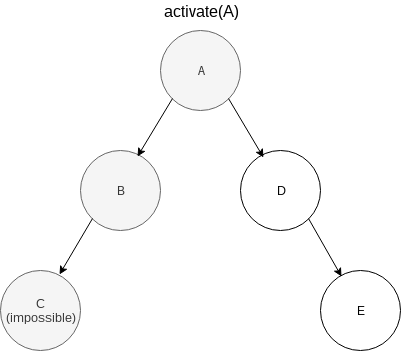
\includegraphics[width=0.5\textwidth]{figures/activate}
  \caption{Activating a district A with one path to a district that can't be activated and one path without problems.}\label{fig:activate}
\end{figure}

\paragraph{Entering a district} This sends a call to the district, passing the creature wanting to enter. The district simply checks to see if the reference is already a key in the creature map, and if not, applies the \texttt{entering}-trigger to the creature entering and the creatures already in the district. The result then represents the  new map of creatures in the state data.

The way the well-formedness of the trigger is checked is as follows. A new process applying the trigger is spawned, which sends a message back with the result. This allows me to use the \texttt{after}-timeout when receiving the result. If there is no result within 2 seconds, the input to the trigger is simply returned. The spawned process calls the trigger and catches any exception that may occur --- if this happens, the input is returned. If there is a response within 2 seconds, the check proceeds by ensuring that the result is a tuple, and that all the creature references are the same. If all is well, the new data is returned. There is no check on the use of functions inside the trigger, so it is possible for trigger to call an API function. This may cause problems if a district applies a trigger that makes a call to this very district, perhaps blocking the process.

\paragraph{Taking action} This sends a call to the district, passing the creature reference and the action. The district makes sure that the creature is actually in the map of contained creatures and that the action exists in the map over neighbours. If so, the \texttt{leaving}-trigger is applied to the creature leaving and the creatures staying in the district, and \texttt{enter} is called on the destination. If all goes well, the creature is moved. One special case is when the action is an edge to the same district; this would, again, block everything. Thus, if the destination is the same as the current district, the \texttt{entering}-trigger is applied locally and the state data is updated accordingly.

This solution may not be the most elegant since it repeats some code from \texttt{enter}. However, given the problems that arise when handling self loops, this solution is a very simple way to avoid blocking the process.

\paragraph{Shutting down a district} This works much in the same way as \texttt{activate}. After sending the required message to the \texttt{NextPlane} argument, the district immediately goes to the \texttt{shutting\_down} state and forces an internal event that makes it shut down its neighbours. After they have all been visited, It uses the \texttt{gen\_statem:stop} to actually terminate the process.




\subsection*{Testing \texttt{district}}

I have already gone over some reasons why my implementation should behave correctly. To further ensure the behavour of my implementation, I have written some unit tests and some property-based tests.

\paragraph{Unit testing} I have chosen to do a series of unit tests much like I did in Haskell. In case the property-based QuickCheck tests are not producing good enough instances, at least these unit tests can tell a bit about the integrity of each part of the implementation. I chose to use EUnit for this task, since it is simple and easy to use, and its error messages when tests fail are very helpful.

There are 50 unit tests which, collectively, cover all requirements from the assignment. These range from connecting districts, moving a creature from a district to another, activating territories with cycles and self loops, registering well-formed triggers and triggers returning ill-formed data and throwing exceptions, and shutting down while checking the messages afterwards. In my opinion, these tests show that the behaviour of my implementation is at least pretty close to the intended behaviour described in the assignment. The fact that all tests pass indicates that a large portion of the solution is correct. The tests can be found in \texttt{ravnica/district\_bb}.


\paragraph{QuickChecking the properties} I have written a territory generator that simply creates a random map as described in the assignment. I have also, as was the task, implemented \texttt{setup\_territory}, which takes this map and creates a district for each of the keys, creates all connections from the \texttt{\{atom(),key()\}} list, and finally returns all district pids as the resulting territory. I won't go into detail about the concrete implementations of these. An example of a generated territory (on the form before setting up the actual districts) can be seen in Appendix \ref{app:genter}. \\

\noindent In order to check the neighbours of and the creatures in the districts after calling som API function, I initially used \texttt{sys:get\_state}. However, I realized that this is heavily implementation-specific (how is the state data represented?), so I had to choose a much simpler, and not as flexible, approach.
Thus, I have implemented property-based for three API functions:
\begin{itemize}
  \item \texttt{activate}
  \item \texttt{shutdown}
  \item \texttt{take\_action}
\end{itemize}
When testing activation, I simply make sure that if we can successully activate some district in the generated territory, then the neighbours will be active afterwards. This is done by creating a creature and moving it to the neighbours. This gives me the pid of the neighbour, and I check the state using \texttt{sys:get\_state} (not relying on the state data, only the state itself). I could assume that moving the creature would be enough since it is only allowed when both the current district and the neighbour are active, but actually fetching the state is in my opinion a better indicator.

When testing the territory when shutting down, I activate some district in the generated territory, create a creature, move it to some neighbour, get the pid of said neighbour, shut down the current district, and check that both processes have terminated using \texttt{process\_info}. This would indicate that a district is actually correctly shut down.

When testing actions, I simply create a creature, enter it in some district from the generated territory, move it to a neighbour through an action, and then try to move it from the same district to a neighbour through the same action. This should fail, since the creature is no longer in the inital district.

\paragraph{Assessment} I realize that my specific property-based tests are not a sure guarantee that my implementation is perfect; they are rather simple, only testing within a very local neighbourhood in any generated territory. However, they still do show some qualities about my implementation that are required in a correct solution, so they are in my opinion far from worthless.

The unit tests, on the other hand, strongly indicate correct behaviour on various instances with intentional edge cases and errors. Here, not a single instance behaves unexpectedly as long as it is well-formed as per the assignment.



% Appendix
\newpage
\appendix

\section{\texttt{appm} listings}
\subsection{Source listings}
\subsubsection{Source code for \texttt{/handin/appm/src/Defs.hs}}
\lstinputlisting[language=haskell]{../handin/appm/src/Defs.hs}
\subsubsection{Source code for \texttt{/handin/appm/src/Utils.hs}}
\lstinputlisting[language=haskell]{../handin/appm/src/Utils.hs}
\subsubsection{Source code for \texttt{/handin/appm/src/ParserImpl.hs}}
\lstinputlisting[language=haskell]{../handin/appm/src/ParserImpl.hs}
\subsubsection{Source code for \texttt{/handin/appm/src/Parser.hs}}
\lstinputlisting[language=haskell]{../handin/appm/src/Parser.hs}
\subsubsection{Source code for \texttt{/handin/appm/src/SolverImpl.hs}}
\lstinputlisting[language=haskell]{../handin/appm/src/SolverImpl.hs}
\subsubsection{Source code for \texttt{/handin/appm/src/Solver.hs}}
\lstinputlisting[language=haskell]{../handin/appm/src/Solver.hs}
\subsubsection{Source code for \texttt{/handin/appm/src/Main.hs}}
\lstinputlisting[language=haskell]{../handin/appm/src/Main.hs}

\subsection{Black-box test listings}
\subsubsection{Source code for \texttt{/handin/appm/tests/BB/UtilTest.hs}}
\lstinputlisting[language=haskell]{../handin/appm/tests/BB/UtilTest.hs}
\subsubsection{Source code for \texttt{/handin/appm/tests/BB/ParserTest.hs}}
\lstinputlisting[language=haskell]{../handin/appm/tests/BB/ParserTest.hs}
\subsubsection{Source code for \texttt{/handin/appm/tests/BB/SolverTest.hs}}
\lstinputlisting[language=haskell]{../handin/appm/tests/BB/SolverTest.hs}
\subsubsection{Source code for \texttt{/handin/appm/tests/BB/Main.hs}}
\lstinputlisting[language=haskell]{../handin/appm/tests/BB/Main.hs}


\subsection{QuickCheck listings}
\subsubsection{Source code for \texttt{/handin/appm/tests/QC/Gen.hs}}
\lstinputlisting[language=haskell]{../handin/appm/tests/QC/Gen.hs}
\subsubsection{Source code for \texttt{/handin/appm/tests/QC/Properties.hs}}
\lstinputlisting[language=haskell]{../handin/appm/tests/QC/Properties.hs}
\subsubsection{Source code for \texttt{/handin/appm/tests/QC/Main.hs}}
\lstinputlisting[language=haskell]{../handin/appm/tests/QC/Main.hs}

\subsection{Other}
\subsubsection{Automatically generated database}\label{app:gendb}
\lstinputlisting{figures/gen.db}

\newpage
\section{Ravnica listings}
\subsection{Source listings}
\subsubsection{Source code for \texttt{/handin/ravnica/district.erl}}
\lstinputlisting[language=erlang]{../handin/ravnica/district.erl}
\subsubsection{Source code for \texttt{/handin/ravnica/the\_diamond\_path.erl}}
\lstinputlisting[language=erlang]{../handin/ravnica/the_diamond_path.erl}
\subsubsection{Source code for \texttt{/handin/ravnica/a\_day\_at\_diku.erl}}
\lstinputlisting[language=erlang]{../handin/ravnica/a_day_at_diku.erl}

\subsection{QuickCheck listings}
\subsubsection{Source code for \texttt{/handin/ravnica/district\_qc.erl}}
\lstinputlisting[language=erlang]{../handin/ravnica/district_qc.erl}

\end{document}
